\section{实验过程}

\subsection{词典的构建}

\subsubsection{词典的生成}

由于语料库开头的时间仅作为标记出现,是一个无意义的符号,因此不将其加入词典。
其余词均加入词典,并同时统计各个词出现的词频。

词典将根据199801\_segpos.txt进行训练,这个训练集是UTF-8编码的。
在NaturalLanguageProcessingLabs/下
运行gen\_dic.py即可得到机械匹配分词使用的词典为dic.txt,
运行gen\_bi\_dic.py即可得到二元文法分词使用的词典bi\_dic.txt。

\subsubsection{词典的格式}

词典编码为UTF-8。其中
dic.txt包含两列,每一行的第一列是词,第二列是对应的词频。
bi\_dic.txt包含两列,每一行的第一列是\textbf{前缀词-当前词},两个词中间用横线“-”
隔开。句首符号BOS用“>”表示,句尾符号EOS用“<”表示。第二列是对应出现的频率。

\subsubsection{词典的分析}

由于需要对词频进行储存,因此词频的加入不会改变实验前4部分的分词结果,反而会降低实验时间性能。

由于在后续阶段使用Hashmap进行词典的存储,因此词典在文件中不需要根据词频进行排序。
这一选择可以提高生成词典时的时间性能。

\subsection{正反向最大匹配分词的实现}

正反向分词的最大匹配实现是基于一个基本思想:
将文本中的和字典匹配的最长词切分出来\citep{张磊2009中文分词算法解析}。

\subsubsection{正反向最大匹配分词流程}

前向最大匹配分词(FMM)流程图如图\ref{fmm},将测试文本的每行作为循环内容,按照词典中的词长
从大到小的顺序依次对每行从前向后进行匹配,若匹配不成功则减小词长重新匹配。

\begin{figure}[H]
  \centering
  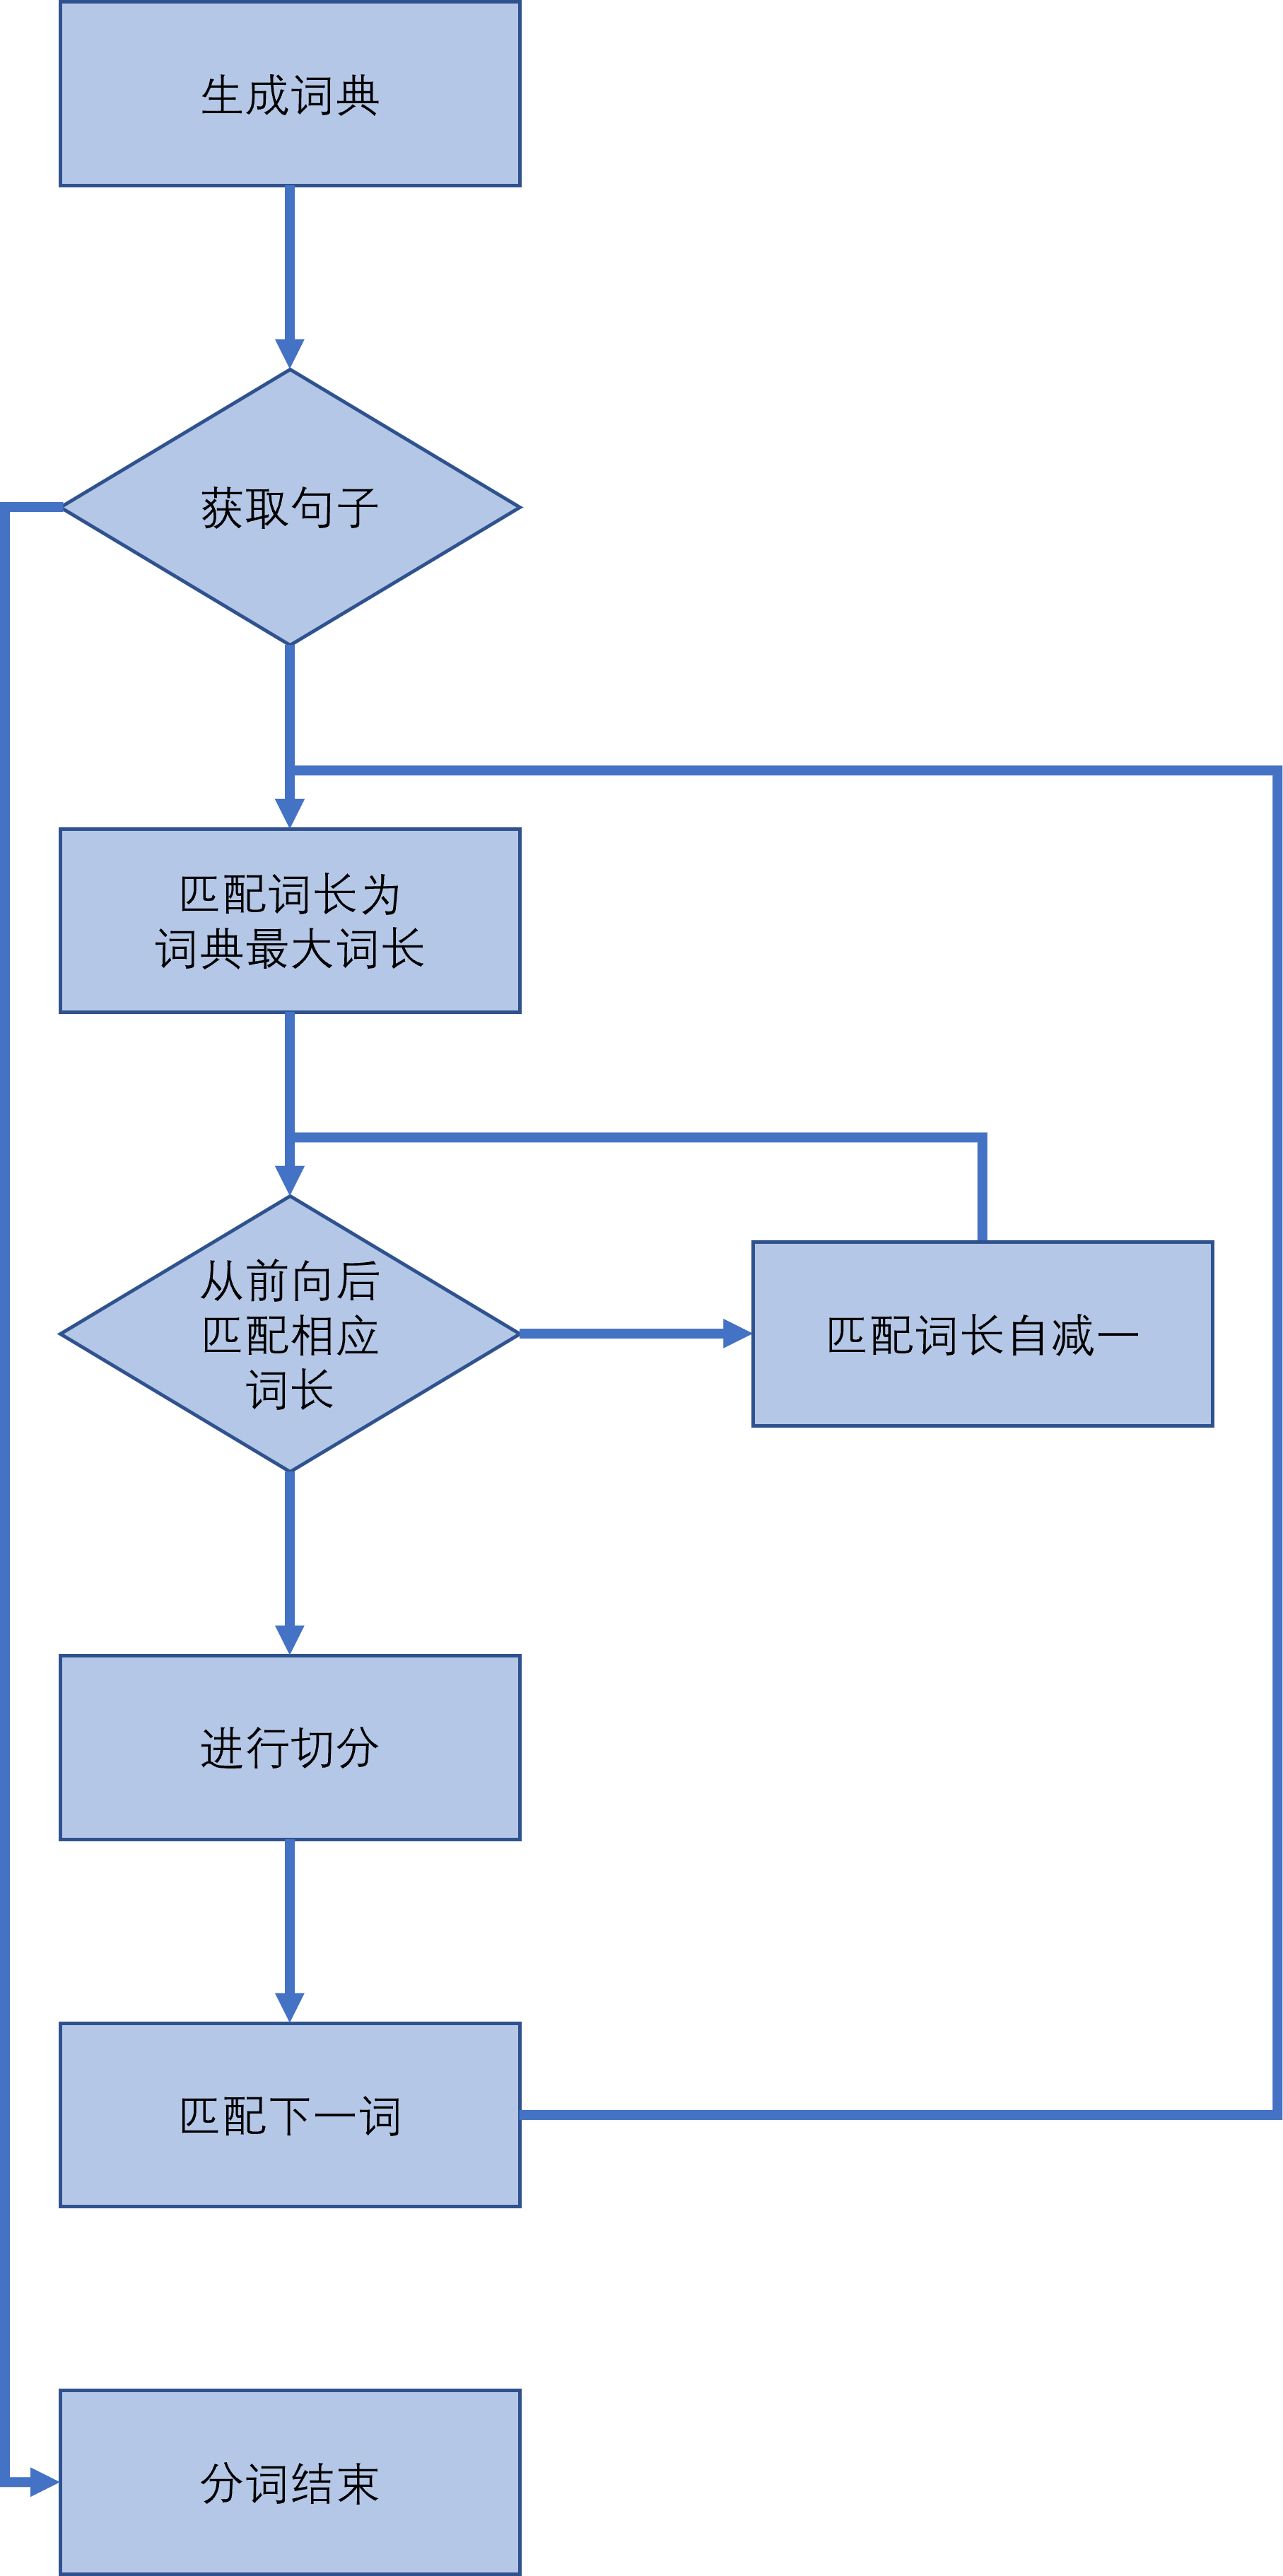
\includegraphics[width=0.3\textwidth]{figures/figure_01.png}
  \caption{前向最大匹配FMM流程图}
  \label{fmm}
\end{figure}

反向最大匹配(BMM)的逻辑与前向最大匹配类似,但是是对每行从后向前进行匹配。
在代码实现时,可以对已经实现的FMM稍作修改,使其从后向前匹配,
并使用栈对匹配结果进行倒序输出即可。

\subsubsection{时间性能}

由于要求最少代码量,因此采取直接将全部词典读入数组中,在查找时直接进行简单的线性搜索。
这个方法时间性能极差,使用Intel Core i7 11700单核运行C语言编写的程序,
将全部测试集分词完毕需要大约22小时。

由于使用C语言而非Python等更高级语言,因此处理字符串的代码量较大,max\_match.c达到262行。

\subsubsection{收获}

最简单的代码思路往往无法直接解决问题,需要在基础思路上做一些优化。

在Python等封装层次很高的语言中,一个字符是Unicode标准的字符,即字母'A'和汉字'中'等均被
识别成一个字符,所以可以方便地进行字符串切片等操作。而在C语言中,一个字符就是一个字节,只能
表示ASCII码以内的字母和控制字符等。而对于UTF-8编码的汉字,一个字可能占2至4个字节,这对
字符串操作有着一定挑战。

因此在实验中专门实现了一个字符串库str.h,重点功能是将读入的UTF-8编码汉字转换为小端UTF-16
编码\citep{garfinkel2013detecting}汉字,从而存放在wchar类型的宽字符数组中,同时在库中
实现了几个专门针对宽字符串wcs的操作函数。

\subsection{正反向最大匹配分词的效果分析}

\subsubsection{原理}

分词效果分析一般使用准确率、召回率及二者的调和平均数F值进行评价。

对于二分类问题,根据真实情况与预测结果的不同组合,分类结果可以分为表\ref{TPFPFNTN}中的4类
\begin{table}[H]
  \centering
  \begin{tabular}{rrr}
    \hline
    \textbf{}    & \textbf{预测结果为正} & \textbf{预测结果为负} \\
    \hline
    真实结果为正 & TP                    & FN                    \\
    真实结果为负 & FP                    & TN                    \\
    \hline
  \end{tabular}
  \caption{二分类问题4种可能性组合}
  \label{TPFPFNTN}
\end{table}

则准确率、召回率及F值计算方法为
\begin{align}
  precision   & = \frac{TP}{TP + FP}                                            \\
  recall      & = \frac{TP}{TP + FN}                                            \\
  \frac{1}{F} & = \frac{1}{2} \left(\frac{1}{precision}+\frac{1}{recall}\right)
\end{align}

以计算准确率为例,其等价于寻找分词结果中正确的比例。借鉴滑动窗口,构造如下算法:
当分词结果与标准结果对应位置相同时,认为分词正确;

\begin{figure}[H]
  \centering
  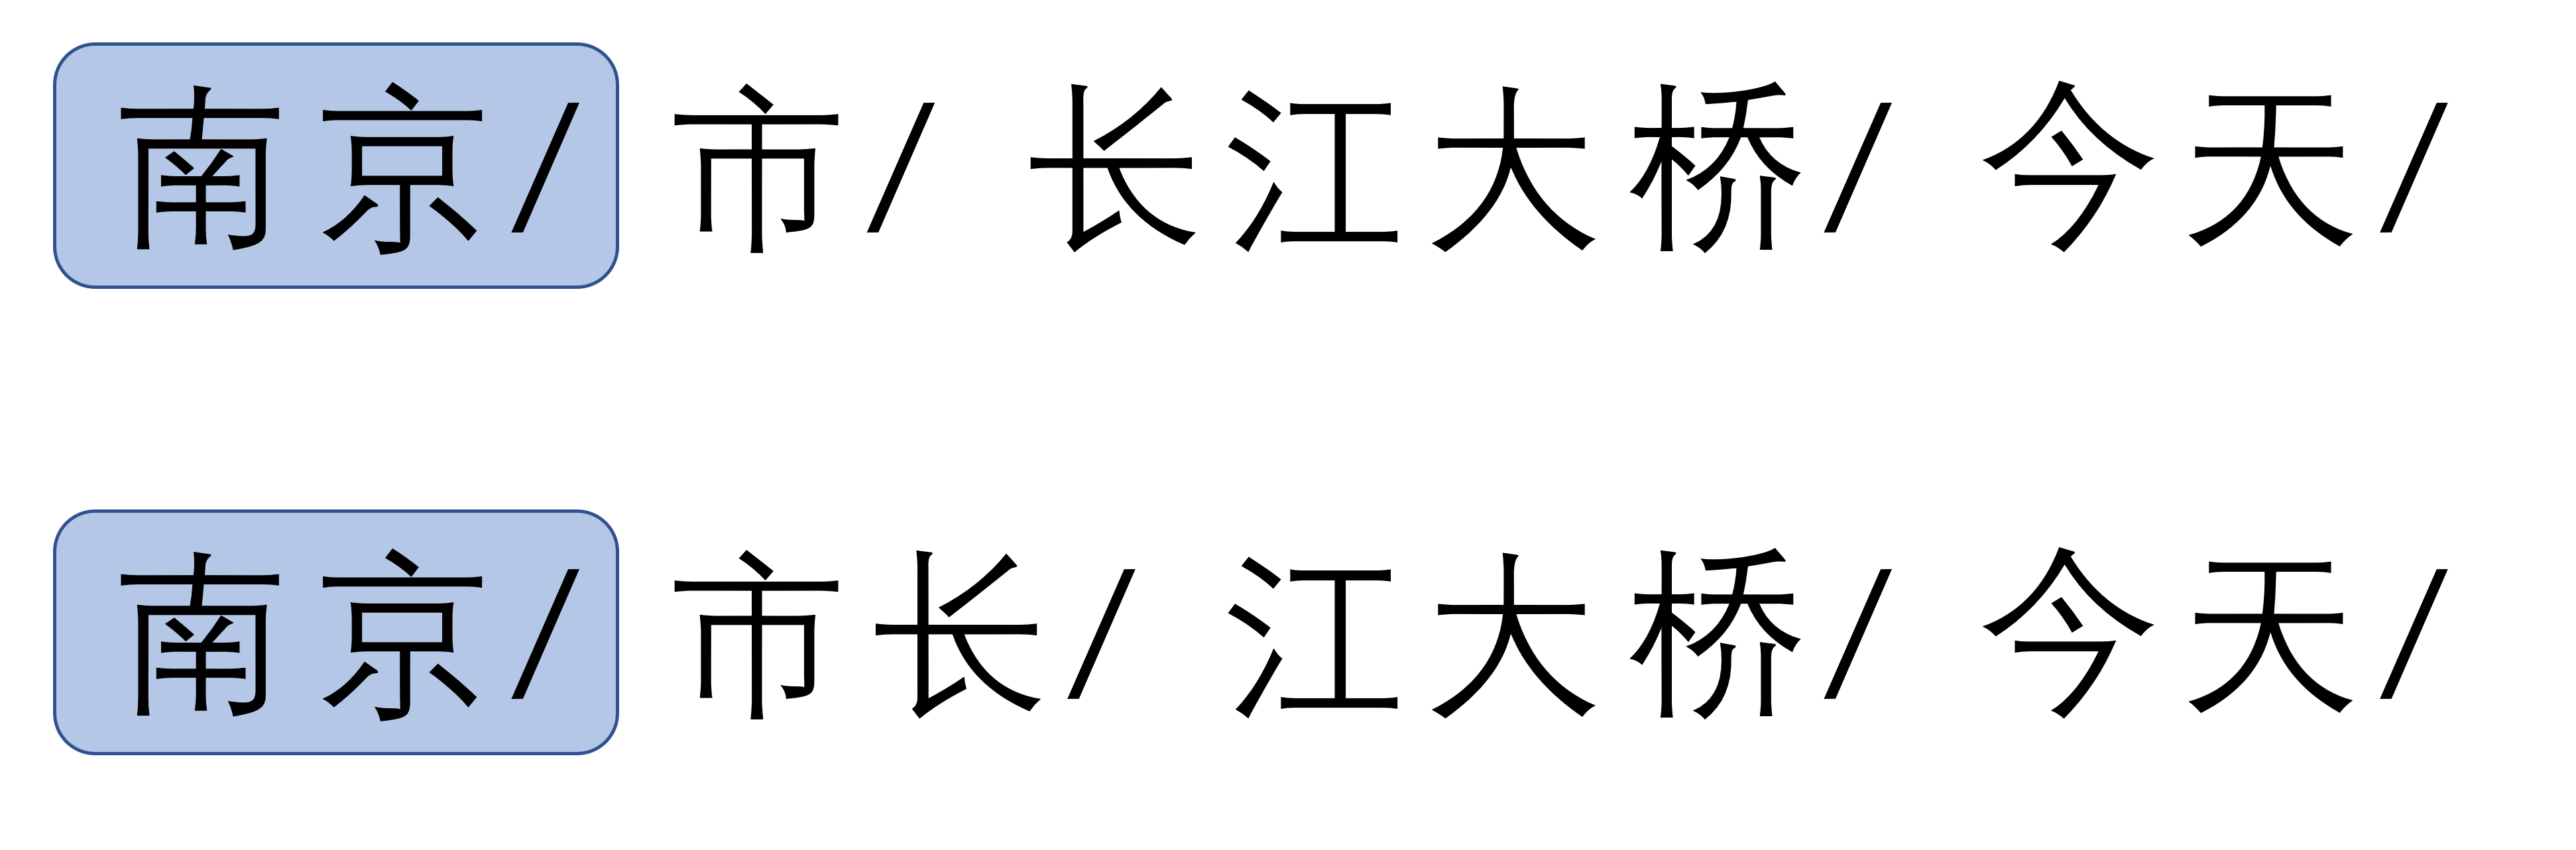
\includegraphics[width=0.3\textwidth]{figures/figure_02.png}
  \caption{对应位置相同,则分词正确}
\end{figure}

当分词结果与标准结果对应位置不同时,则此处分词不正确,同时说明后续一定存在分词不正确的位置;

\begin{figure}[H]
  \centering
  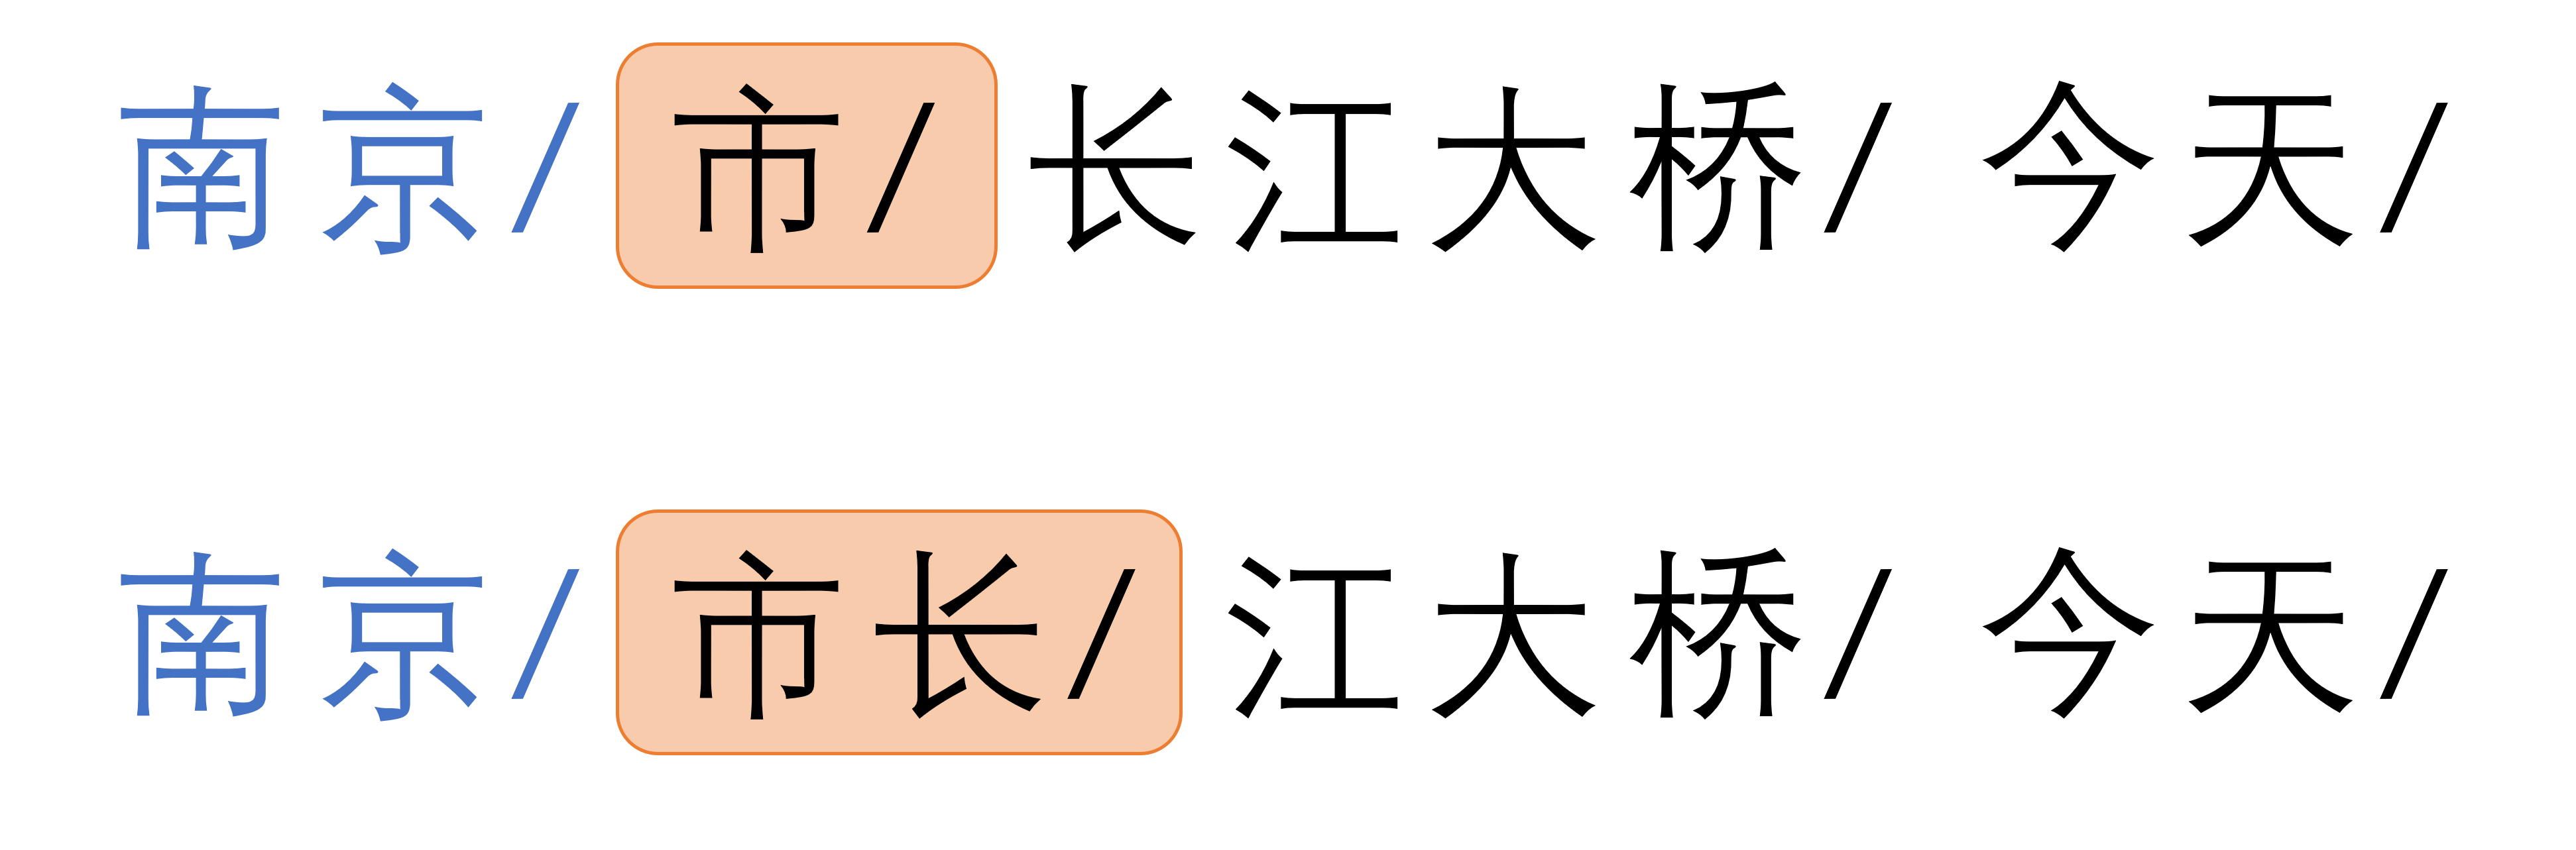
\includegraphics[width=0.3\textwidth]{figures/figure_03.png}
  \caption{对应位置不同,此处分词不正确,同时后续一定也存在不正确}
\end{figure}

此时分词结果和标准结果分别向后扩大窗口范围,直到找到匹配的字符串。
此时,窗口内的所有字符串都属于分词错误,下一次匹配应该从窗口末端开始。

\begin{figure}[H]
  \centering
  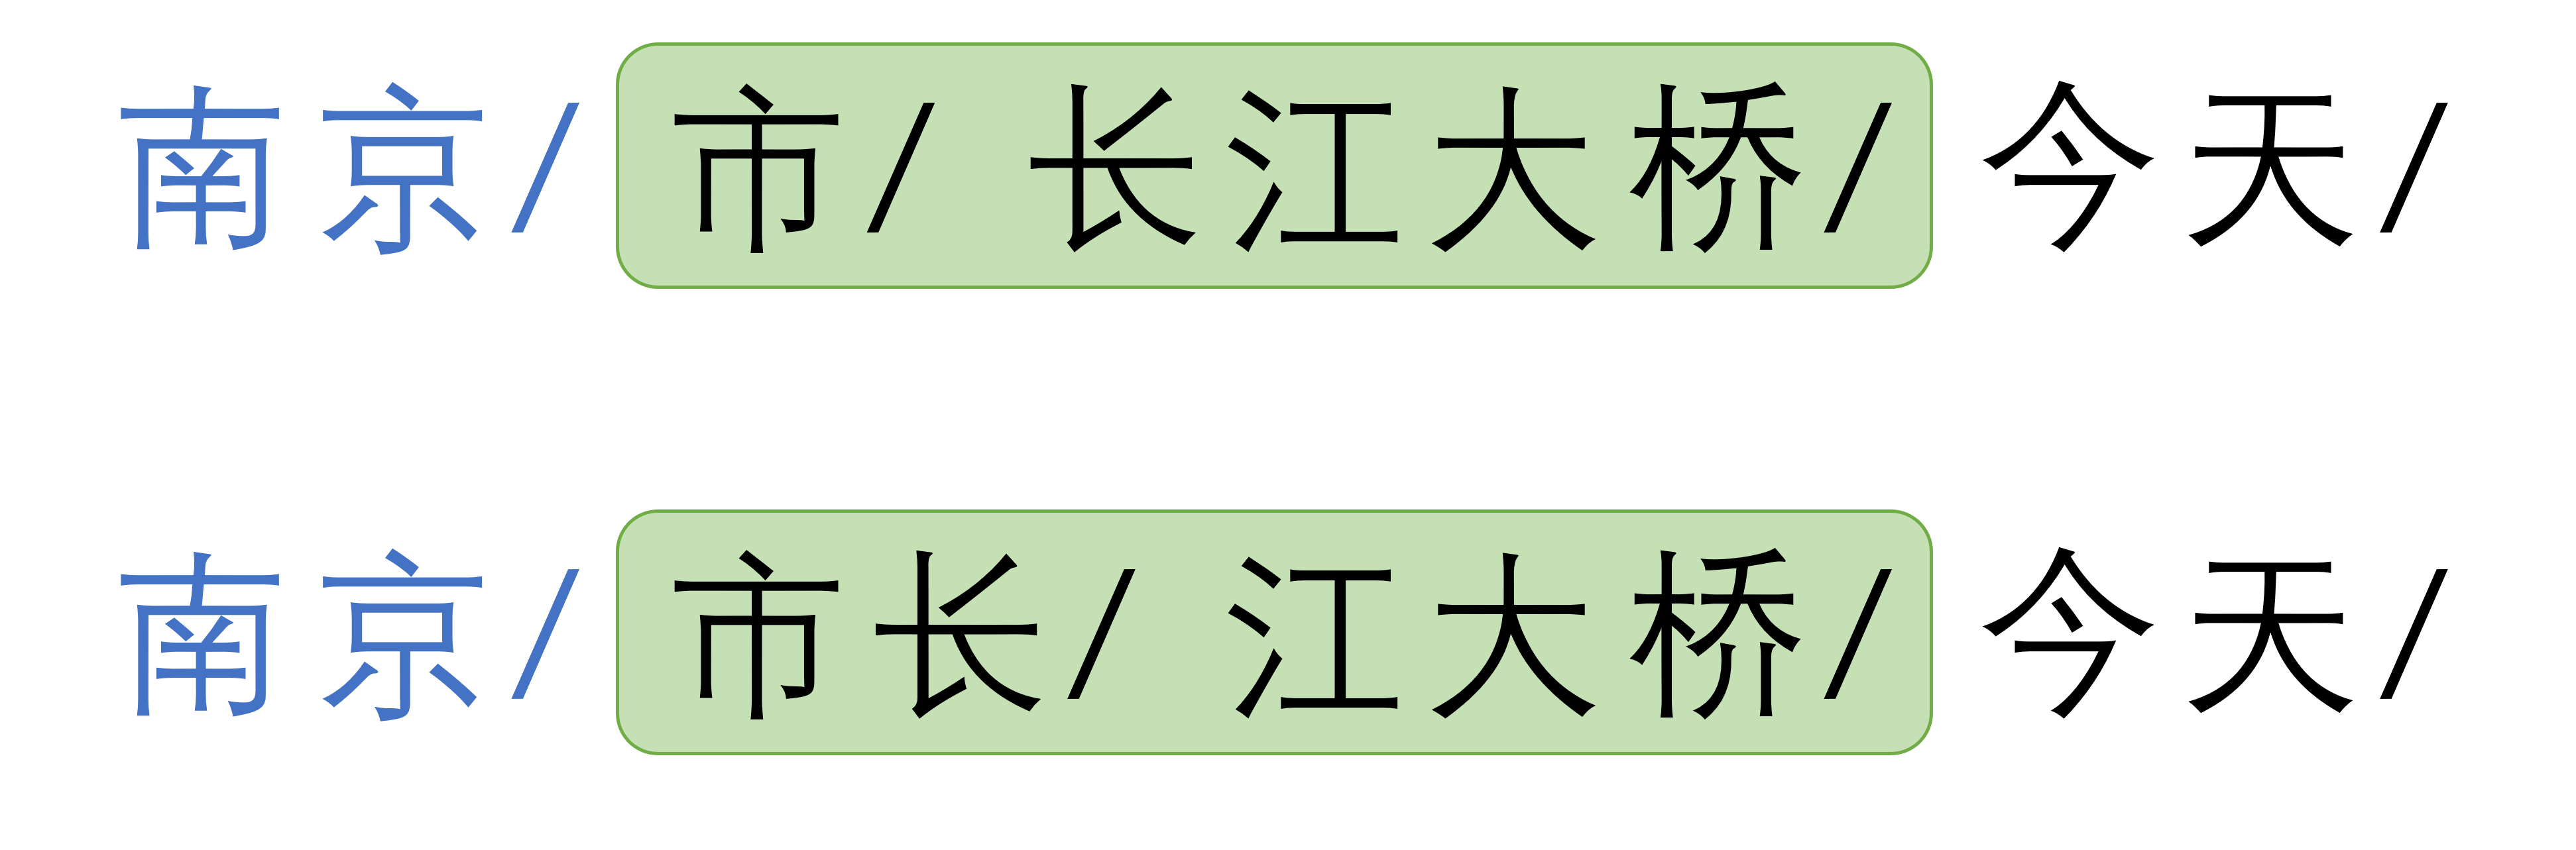
\includegraphics[width=0.3\textwidth]{figures/figure_04.png}
  \caption{向后扩大窗口范围找到匹配的字符串}
\end{figure}

接下来跳转到算法起始位置,重新开始匹配字符串,检验分词是否正确

\begin{figure}[H]
  \centering
  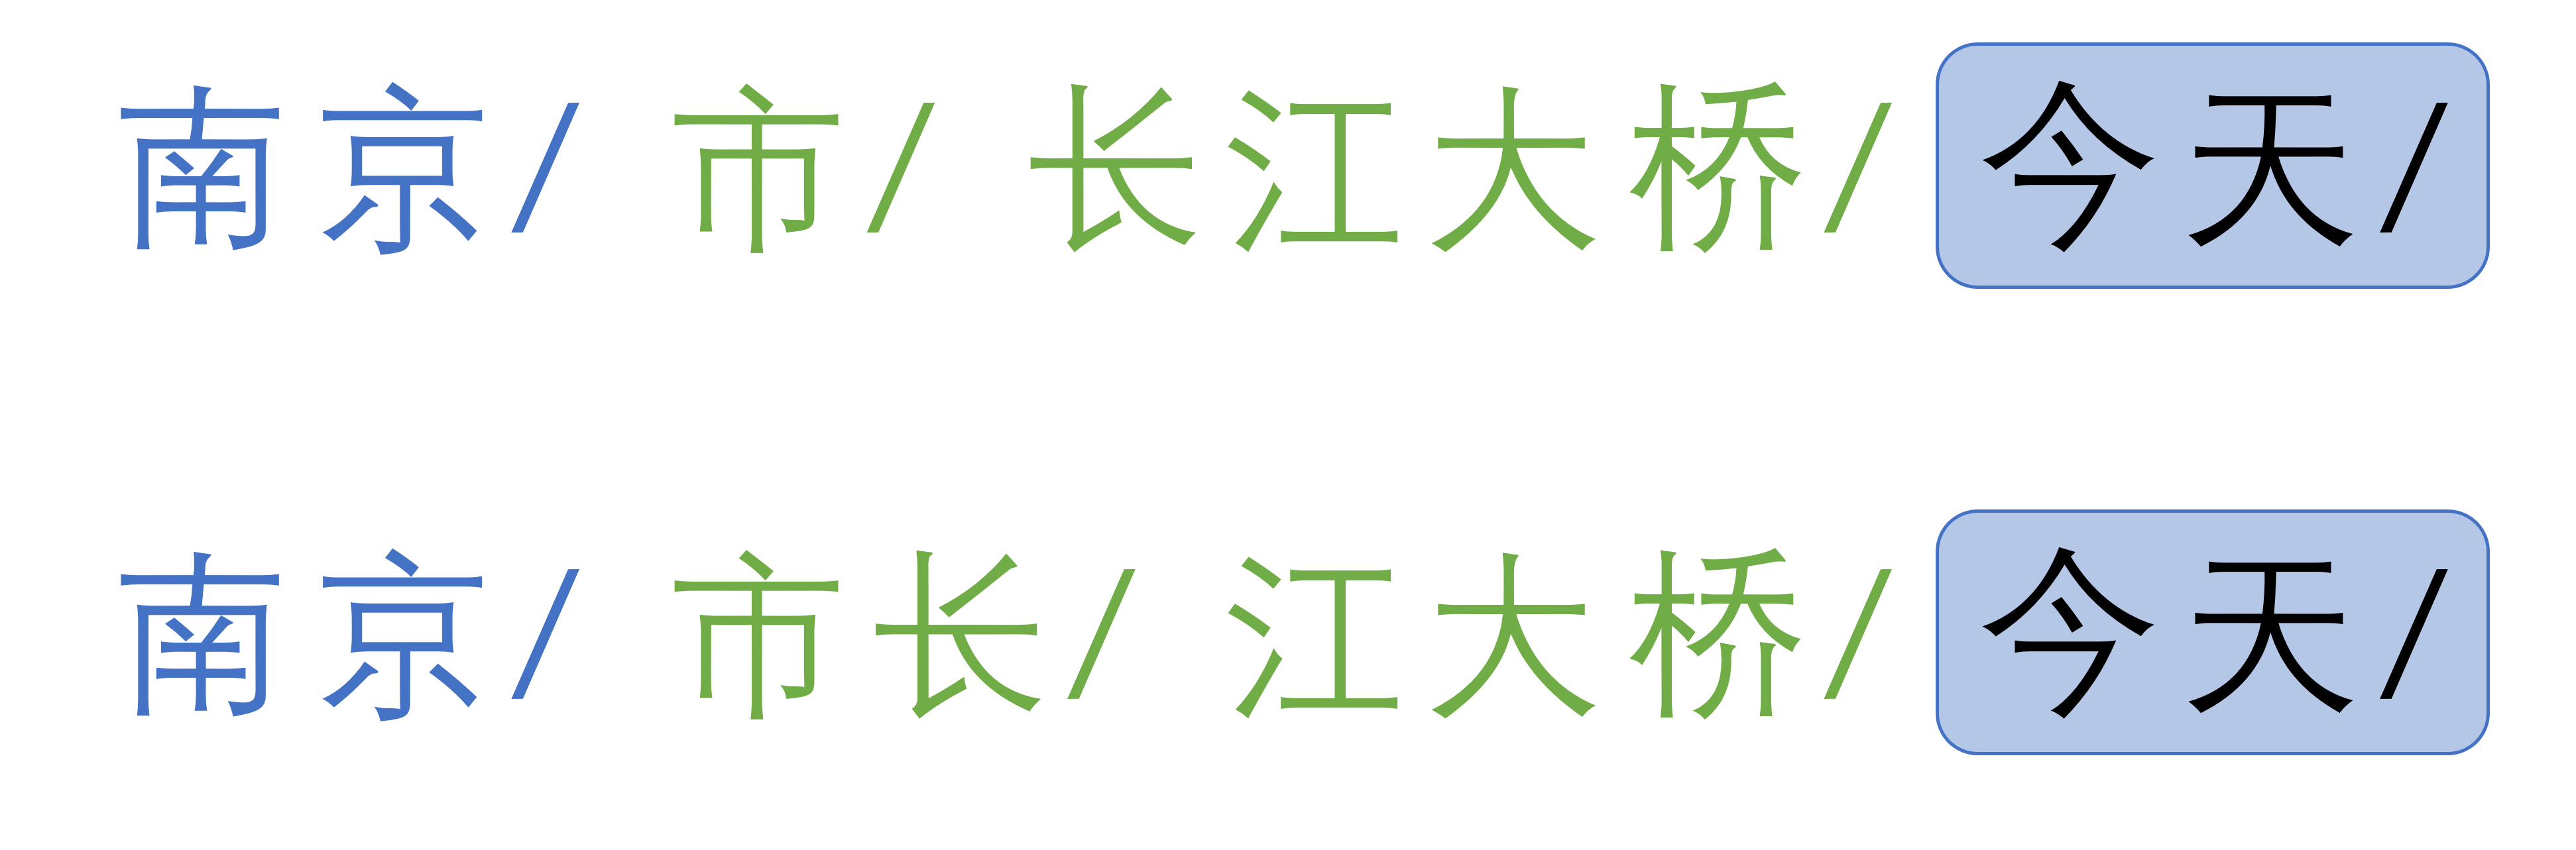
\includegraphics[width=0.3\textwidth]{figures/figure_05.png}
  \caption{重新开始匹配字符串}
\end{figure}
\begin{figure}[H]
  \centering
  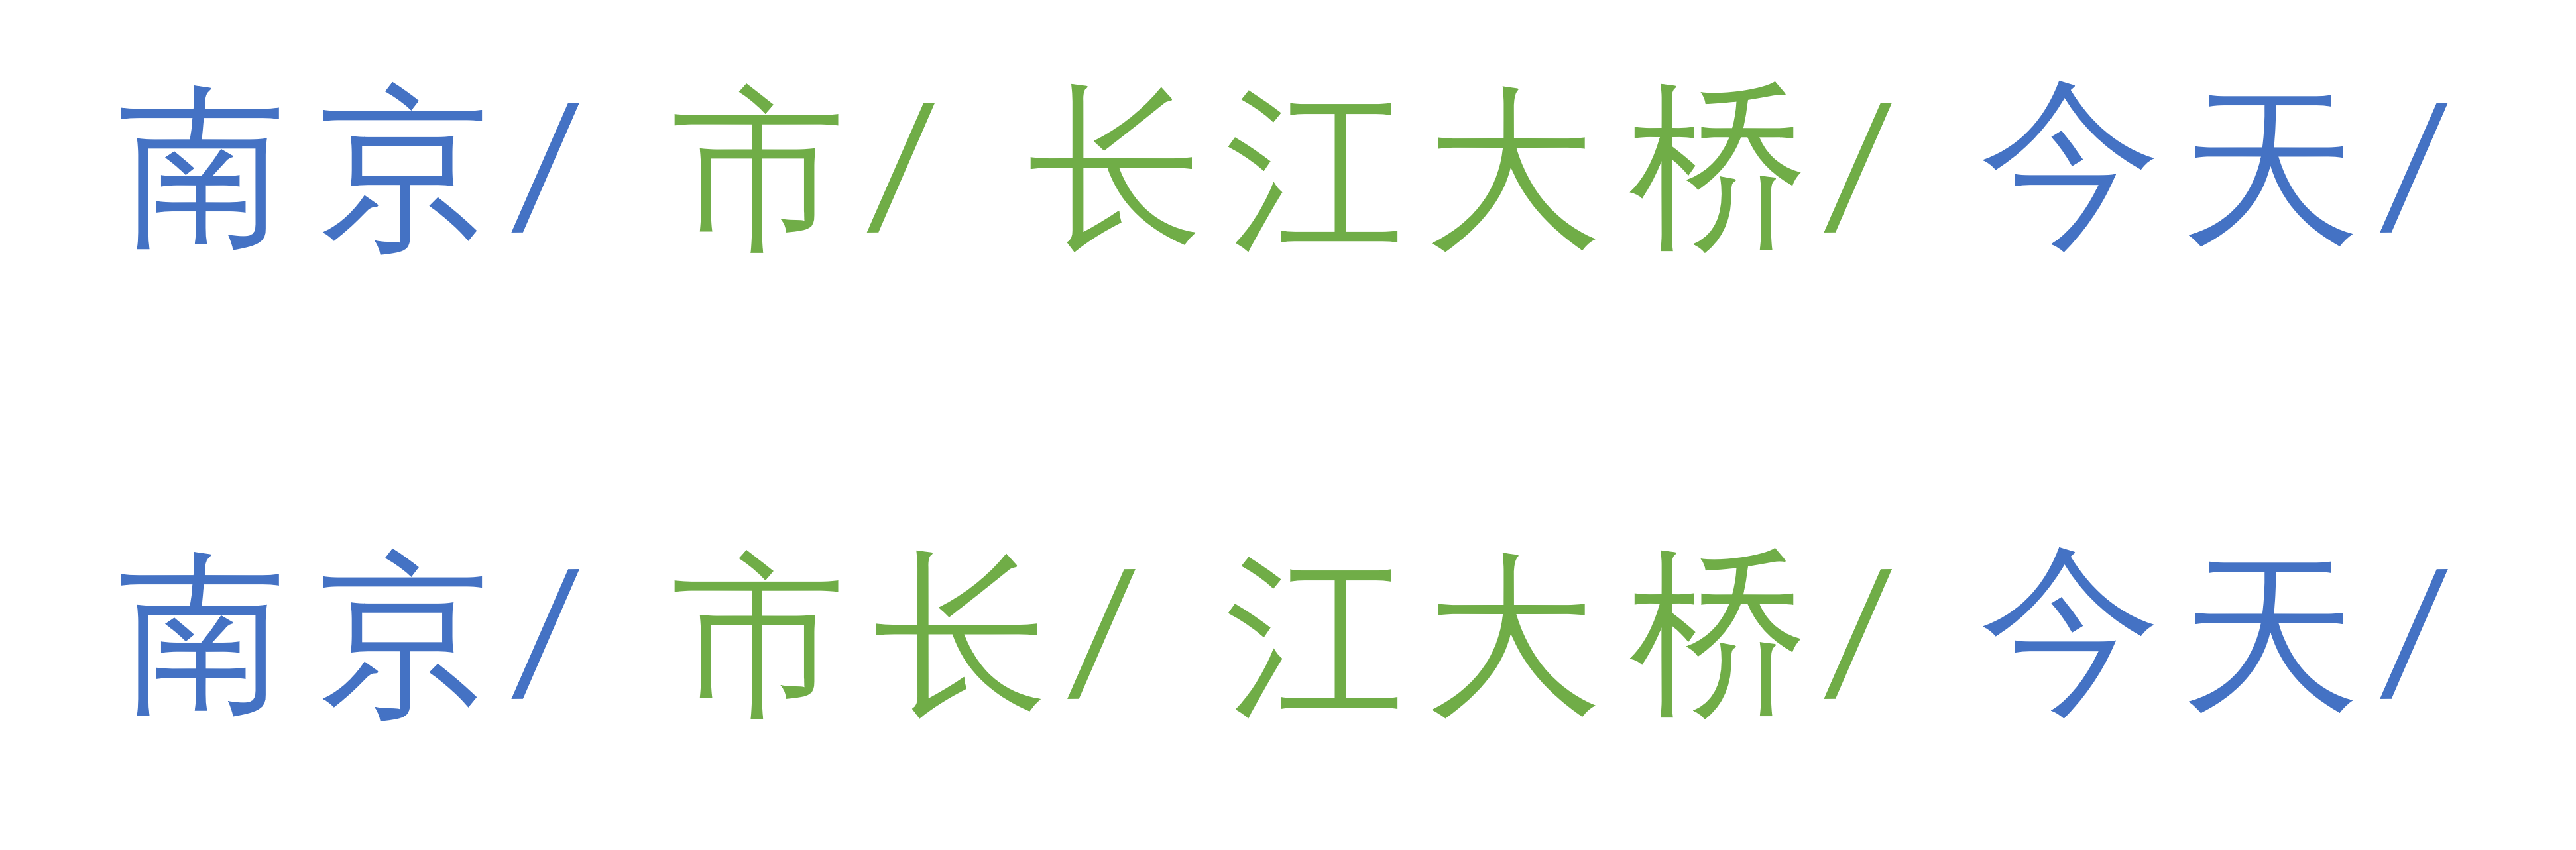
\includegraphics[width=0.3\textwidth]{figures/figure_06.png}
  \caption{检验到句尾,则结束检验}
\end{figure}

\subsubsection{实际分析}

采用类滑动窗口算法,得到FMM和BMM分词性能表\ref{seg_evaluate}

\begin{table}[H]
  \centering
  \begin{tabular}{lrr}
    \hline
    \textbf{性能} & \textbf{FMM} & \textbf{BMM} \\
    \hline
    Precision     & 97.8\%       & 98.0\%       \\
    Recall        & 97.1\%       & 97.3\%       \\
    F             & 97.5\%       & 97.6\%       \\
    \hline
  \end{tabular}
  \caption{FMM和BMM分词性能对比}
  \label{seg_evaluate}
\end{table}

可见BMM在准确率和召回率都稍稍优于FMM。

从直观分析,对于汉语的一个词,在这个词后边加一个字仍能构成词的频率较高,而在这个词前边加
一个字仍能构成词的频率较低。
因此FMM更容易将标准词前边的词加入到分词结果中,导致标准词被错误切成多个词,而相较而言BMM
则更容易匹配到正确的词。

\subsection{机械匹配的分词系统的速度优化}

在最短代码实现正反向最大匹配中,查找词典使用的是$O(n)$复杂度的线性查找。
可以采用HashMap对查找进行速度优化,时间复杂度可降至$O(1)$。

HashMap的关键是构造哈希函数,借鉴JDK 1.7的哈希函数构造方法,
可以构造字符串的哈希函数:对字符串中的每个字符c,都有
\begin{equation}
  \label{hash31}
  hash = 31 \times hash + c
\end{equation}
在遍历每个字符串后,对哈希值进一步操作
\begin{equation}
  hash = hash \oplus (hash >> 16)
\end{equation}
即可得到这个字符串的哈希值。伪代码如算法\ref{hashcode-algorithm}所示。
\begin{algorithm}
  \caption{Hash Code}
  \begin{algorithmic}
    \STATE $hash \gets 0$
    \STATE $c \gets string_{start}$
    \WHILE{$c \neq string_{end}$}
    \STATE $hash \gets 31 \times hash + c$
    \STATE $c \gets c_{next}$
    \ENDWHILE
    \STATE $hashcode \gets hash \oplus (hash >> 16)$
  \end{algorithmic}
  \label{hashcode-algorithm}
\end{algorithm}

此方法可以较大程度上减少哈希碰撞\citep{bajracharyareview}。
在Intel Core i7 11700机器上,使用线性搜索和HashMap搜索的正反向最大匹配分词
所用时间如表\ref{plain_vs_hashmap_time}。

\begin{table}[H]
  \centering
  \begin{tabular}{lrr}
    \hline
    \textbf{搜索算法} & \textbf{FMM} & \textbf{BMM} \\
    \hline
    BF                & 82419.7s     & 97404.3s     \\
    HashMap           & 6.6s         & 7.8s         \\
    \hline
  \end{tabular}
  \caption{使用线性搜索和HashMap的时间对比}
  \label{plain_vs_hashmap_time}
\end{table}

由表\ref{plain_vs_hashmap_time}可见,使用HashMap将分词速度提高了约12000倍。
但是根据HashMap算法原理中的式\ref{hash31},计算一个字符串的哈希值与字符串长度线性相关,
因此认为HashMap可以实现$O(1)$的查找是不严谨的,其查找速率可以认为是$O(strlen)$。

可以进一步优化HashMap为Trie,这是专门针对字符串进行优化的数据结构\citep{bodon2003trie}。
同时在工程角度可以采用多线程方法,利用现代CPU的多核优势进行速度优化。

\subsection{基于统计的二元文法分词}

\subsubsection{算法思想}

二元文法核心思想是最大化式\ref{bigram}
\begin{equation}
  p\left(w_1|BOS\right) \cdot p\left(w_2|w_1\right) \ldots p\left(EOS|w_n\right)
  \label{bigram}
\end{equation}
其中二元词频为
\begin{equation}
  p\left(w_{i+1}|w_i\right) = \dfrac{\# w_i w_{i+1}}{\sum_{w_i} \# w_i w_{i+1}}
\end{equation}
由于二元文法需要的训练词表大小较一元文法指数级上升,因此需要对二元词频进行一定的平滑处理,
从而在一定程度上缓解词典的稀疏问题。

通常可以采用$\epsilon$-平滑,即
\begin{equation}
  p(w_i|w_{i-1})=\dfrac{f(w_{i-1} w_i)+\epsilon}{f(w_{i-1})+V \epsilon}
\end{equation}

本项目采取的平滑处理为插值法,将一元文法与二元文法线性融合,即
\begin{equation}
  \begin{split}
    p'\left(w_i|w_{i-1}\right)=
    \left(1-\lambda\right)p\left(w_i|w_{i-1}\right)+\\
    \lambda p\left(w_i\right)
  \end{split}
\end{equation}

式\ref{bigram}相当于在有向图中找到最短路径,可以采用Viterbi算法
\citep{forney1973viterbi},即在“篱笆型”图中使用动态规划思想求最短路径。

首先构造有向无环图,我们认为句子中的每一个字之间的空白都是一个节点。
添加有向边的规则为:若一个词在前缀词词典中,则这个词的开始和末尾两个节点添加一条有向边。
基于此规则遍历以每个字开头的可能的词,从而构建出完整的有向图。

\begin{figure}[H]
  \centering
  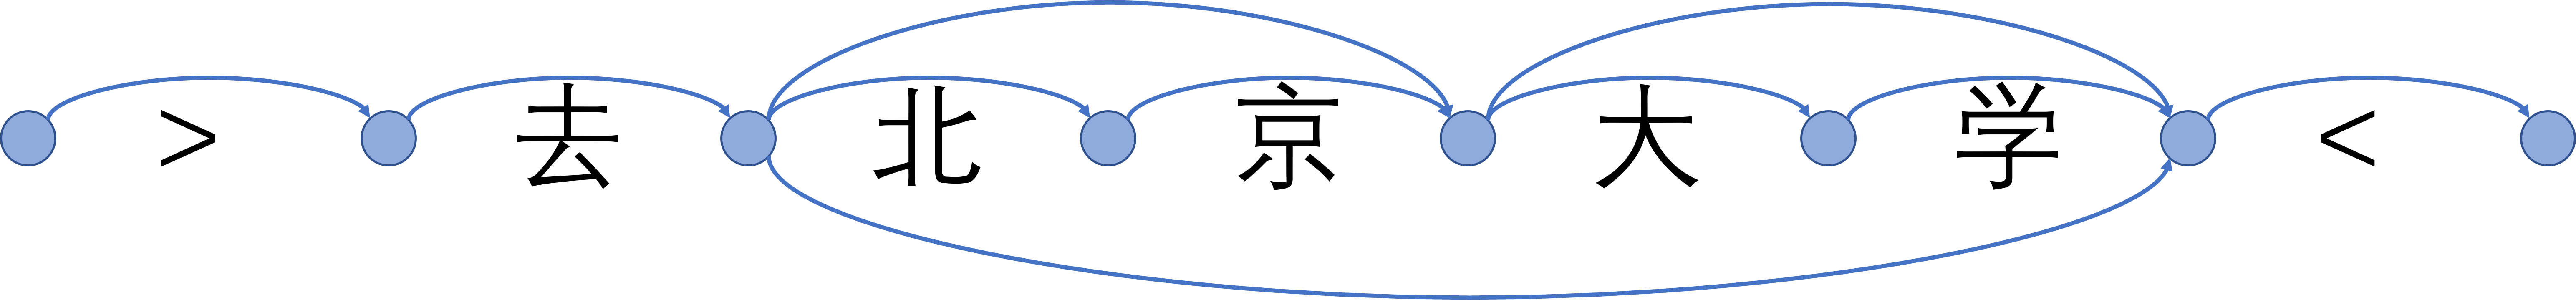
\includegraphics[width=0.4\textwidth]{figures/figure_07.png}
  \caption{构造有向无环图}
\end{figure}

基于动态规划算法,到达一个节点的最小代价,等于到达其前置节点的代价加前置节点到该节点的代价
中的最小值。而在二元文法中,还要更进一步找到前置节点的前置节点,故总的状态转移方程为\ref{dp}
\begin{equation}
  cost_i = \min \{ \log P\left(u \rightarrow i | v \rightarrow u \right) \}
  \label{dp}
\end{equation}
其中$u$是节点$i$的每一个前置节点,而$v$是$u$已经确定最小代价的前置节点。
算法伪代码如\ref{dp_alg}所示。

\begin{algorithm}
  \caption{动态规划搜索最小代价路径}
  \begin{algorithmic}
    \FORALL {$i \in (2, strlen(sentence)+1)$}
    \IF {$rgraph[i]=0$}
    \STATE $prev \gets i-1$
    \ELSIF {$rgraph[i]=1$}
    \STATE $rroute[i] \gets rgraph[i][0]$
    \ELSE
    \FORALL {$prev \in rgraph[i]$}
    \STATE $biword \gets sentence[rroute[prev]:prev]-sentence[prev:i]$
    \STATE $cost \gets possibility[biword]$
    \ENDFOR
    \STATE find max $prev$
    \ENDIF
    \ENDFOR
  \end{algorithmic}
  \label{dp_alg}
\end{algorithm}

由式\ref{dp}中$v$的定义可以看出在这个情境下动态规划是如何加速搜索的,考虑图\ref{p6}情况

\begin{figure}[H]
  \centering
  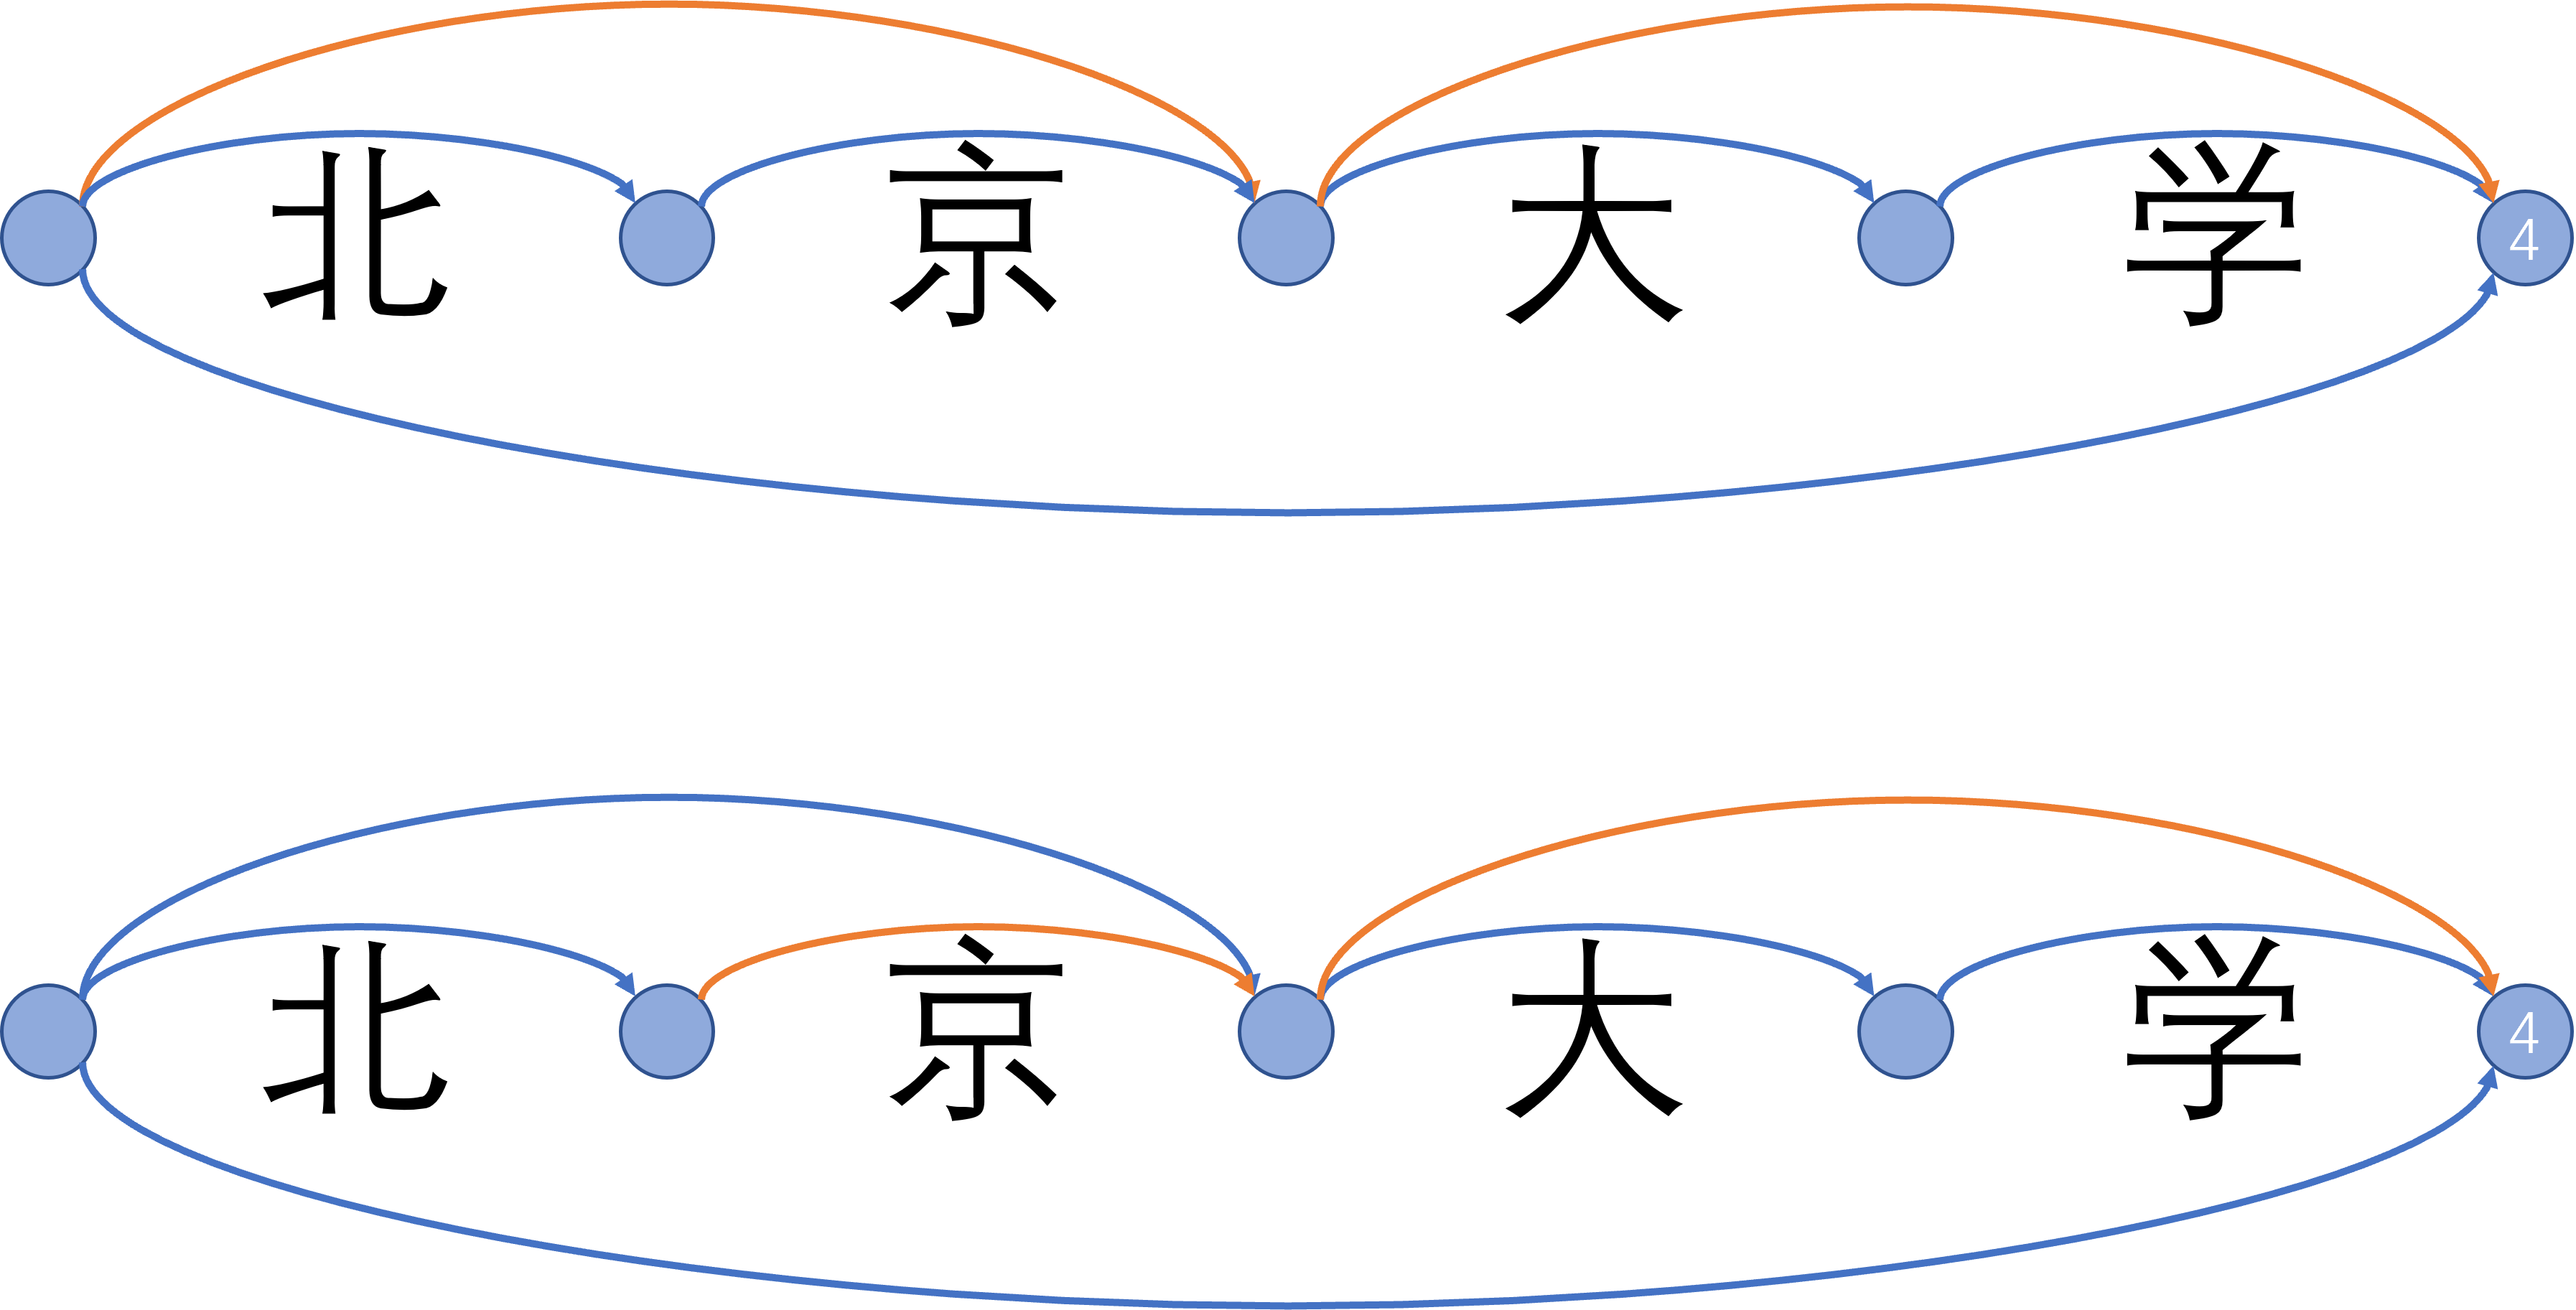
\includegraphics[width=0.3\textwidth]{figures/figure_08.png}
  \caption{前置节点的前置节点的选择}
  \label{p6}
\end{figure}

对于节点4“学$\cdot$EOS”,其有3个前置节点,而对于前置节点“京$\cdot$大”,其又有两个前置
节点“北$\cdot$京”和“BOS$\cdot$北”。若不使用动态规划,则需要分别计算“北$\cdot$京”和
“BOS$\cdot$北”两条路径的总代价;而在动态规划确定了前置节点的最佳前置节点后,则需要计算的
路径数量直接下降为1。从而加速最小代价路径搜索。

\subsubsection{未登录词识别}

采用一种快速的未登录词识别方法:在路径搜索时,若词长为1(即词只有一个字)则将其视为未登录词的
片段;对于连续的未登录词片段(字),视其为一整个未登录词,将其加入词典中并对其进行切分。

\subsubsection{综合性能对比}

使用199801和199802语料库进行训练,并用199801进行性能测试,各个算法性能如表
\ref{seg_evaluate2}所示。

\begin{table}[H]
  \centering
  \begin{tabular}{lrrr}
    \hline
    \textbf{算法} & \textbf{Precision} & \textbf{Recall} & \textbf{F} \\
    \hline
    Uni-gram      & 99.0\%             & 98.2\%          & 98.6\%     \\
    Bi-gram       & 95.6\%             & 97.7\%          & 96.5\%     \\
    Bi-gram UNK   & 95.7\%             & 97.7\%          & 96.7\%     \\
    \hline
  \end{tabular}
  \caption{基于概率的分词模型性能测试}
  \label{seg_evaluate2}
\end{table}

对比可知在当前语料库环境下,一元文法优于二元文法。而当改变语料库为只有199802时,一元文法的
准确率和召回率都有所下降说明一元文法在一定程度上出现了过拟合。二元文法在由于对未登录词的
处理比较粗糙,所以性能比原二元文法并未上升太多,而且由于连续的单独的已登录词被识别成
未登录词,可能导致性能下降。此处可以使用基于HMM的方法对未登录词做进一步精细化处理。
